\documentclass[12pt]{article}

%==============Packages & Commands==============
\usepackage{graphicx}
\usepackage{fancyvrb}
\usepackage{tikz}
%%%<
\usepackage{listings}
%\usepackage[active,tightpage]{preview}
%\PreviewEnvironment{tikzpicture}
%\setlength\PreviewBorder{5pt}%

\usepackage{geometry}                		% See geometry.pdf to learn the layout options. There are lots.
\geometry{letterpaper}                   		% ... or a4paper or a5paper or ...
%\geometry{landscape}                		% Activat\usetikzlibrary{arrows}e for for rotated page geometry
%\usepackage[parfill]{parskip}    		% Activate to begin paragraphs with an empty line rather than an indent
\usepackage{graphicx}				% Use pdf, png, jpg, or eps§ with pdflatex; use eps in DVI mode
								% TeX will automatically convert eps --> pdf in pdflatex
\usepackage{amsmath}
\usepackage{amssymb}

\usepackage[ruled,vlined]{algorithm2e}
\usetikzlibrary{arrows}
\usepackage{alltt}
\usepackage[T1]{fontenc}
\usepackage[utf8]{inputenc}
\usepackage{indentfirst}
\usepackage[longnamesfirst]{natbib} % For references
\bibpunct{(}{)}{;}{a}{}{,} % Reference punctuation
\usepackage{changepage}
\usepackage{setspace}
\usepackage{booktabs} % For tables
\usepackage{rotating} % For sideways tables/figures
\usepackage{amsmath}
\usepackage{multirow}
\usepackage{color}
 
\definecolor{codegreen}{rgb}{0,0.6,0}
\definecolor{codegray}{rgb}{0.5,0.5,0.5}
\definecolor{codepurple}{rgb}{0.58,0,0.82}
\definecolor{backcolour}{rgb}{0.95,0.95,0.92}
 
\lstdefinestyle{mystyle}{
    backgroundcolor=\color{backcolour},   
    commentstyle=\color{codegreen},
    keywordstyle=\color{magenta},
    numberstyle=\tiny\color{codegray},
    stringstyle=\color{codepurple},
    basicstyle=\footnotesize,
    breakatwhitespace=false,         
    breaklines=true,                 
    captionpos=b,                    
    keepspaces=true,                 
    numbers=left,                    
    numbersep=5pt,                  
    showspaces=false,                
    showstringspaces=false,
    showtabs=false,                  
    tabsize=2
}
 
\lstset{style=mystyle}
\usepackage{dcolumn}
\usepackage{comment}
%\usepackage{fullwidth}
\newcolumntype{d}[1]{D{.}{\cdot}{#1}}
\newcolumntype{.}{D{.}{.}{-1}}
\newcolumntype{3}{D{.}{.}{3}}
\newcolumntype{4}{D{.}{.}{4}}
\newcolumntype{5}{D{.}{.}{5}}
\usepackage{float}
\usepackage[hyphens]{url}
%\usepackage[margin = 1.25in]{geometry}
%\usepackage[nolists,figuresfirst]{endfloat} % Figures and tables at the end
\usepackage{subfig}
\captionsetup[subfloat]{position = top, font = normalsize} % For sub-figure captions
\usepackage{fancyhdr}
%\makeatletter
%\def\url@leostyle{%
%  \@ifundefined{selectfont}{\def\UrlFont{\sf}}{\def\UrlFont{\small\ttfamily}}}
%\makeatother
%% Now actually use the newly defined style.
\urlstyle{same}
\usepackage{times}
\usepackage{mathptmx}
%\usepackage[colorlinks = true,
%						bookmarksopen = true,
%						pagebackref = true,
%						linkcolor = black,
%						citecolor = black,
% 					urlcolor = black]{hyperref}
%\usepackage[all]{hypcap}
%\urlstyle{same}
\newcommand{\fnote}[1]{\footnote{\normalsize{#1}}} % 12 pt, double spaced footnotes
\def\citeapos#1{\citeauthor{#1}'s (\citeyear{#1})}
\def\citeaposs#1{\citeauthor{#1}' (\citeyear{#1})}
\newcommand{\bm}[1]{\boldsymbol{#1}} %makes bold math symbols easier
\newcommand{\R}{\textsf{R}\space} %R in textsf font
\newcommand{\netinf}{\texttt{NetInf}\space} %R in textsf font
\newcommand{\iid}{i.i.d} %shorthand for iid
\newcommand{\cites}{{\bf \textcolor{red}{CITES}}} %shorthand for iid
%\usepackage[compact]{titlesec}
%\titlespacing{\section}{0pt}{*0}{*0}
%\titlespacing{\subsection}{0pt}{*0}{*0}
%\titlespacing{\subsubsection}{0pt}{*0}{*0}
%\setlength{\parskip}{0pt}
%\setlength{\parsep}{0pt}
%\setlength{\bibsep}{2pt}
%\renewcommand{\headrulewidth}{0pt}

%\renewcommand{\figureplace}{ % This places [Insert Table X here] and [Insert Figure Y here] in the text
%\begin{center}
%[Insert \figurename~\thepostfig\ here]
%\end{center}}
%\renewcommand{\tableplace}{%
%\begin{center}
%[Insert \tablename~\theposttbl\ here]
%\end{center}}

\newcommand\independent{\protect\mathpalette{\protect\independenT}{\perp}}
\def\independenT#1#2{\mathrel{\rlap{$#1#2$}\mkern2mu{#1#2}}}
\newcommand{\N}{\mathcal{N}}
\newcommand{\Y}{\bm{\mathcal{Y}}}
\newcommand{\bZ}{\bm{Z}}

\usepackage[colorlinks = TRUE, urlcolor = black, linkcolor = black, citecolor = black, pdfstartview = FitV]{hyperref}


%============Article Title, Authors==================
\title{\vspace{-2cm} Testing for Network Effects in Field Experiments: Examples from Legislative Studies } 


\author{ Sayali Phadke \and Bruce Desmarais} \date{\today}



%===================Startup=======================
\begin{document}
\maketitle



%=============Abstract & Keywords==================

\begin{abstract}

\noindent  Most social processes involve complex interaction and dependence among units in a network. The stable unit treatment value assumption (SUTVA)--the assumption that a unit’s outcome is unaffected by other units’ treatment statuses—is required in conventional approaches to causal inference. When SUTVA is violated, as in networked social interaction, treatment effects spread to control units through the network structure. We evaluate the evidence for spillover effects in data from three field experiments on US state legislatures. Randomized field experiments represent the gold standard in causal inference when studying political elites. It is not possible to bring political elites into the lab, and causal identification with observational data is fraught with problems. We propose new specifications for treatment spillover models, and construct networks through geographical or ideological proximity and co-sponsorship. Considering different combinations of spillover models and networks, we evaluate the robustness of recently developed non-parametric tests for interference. The approaches we illustrate can be applied to any experimental setting in which interference is suspected. \\~\\

\end{abstract}
\thispagestyle{empty}
\doublespacing
% Description of the possible challenges
\section{Introduction}

Networks are integral parts of human interaction and hence social science research. If one unit in a network gets treated, the effect may trickle down throughout network. The currently established framework for causal inference relies on SUTVA (Stable Unit Treatment Value Assumprion). It assumes that whether or not one person/unit/node is treated, does not affect any other unit. However, SUTVA breaks down in a network setting. It is therefore imperative to take the interference structure into account. Rather, in policy planning or designing marketing campaigns, a researcher may be interested in studying the propogation of treatment effect itself.

In field experiments on social groups, interference may be substantial. In this project we intend to study intererence models for randomized experiments coducted on social networks and causal inference basis this.

To understand, explain and predict social phenomena, social scientists typically look to individual actors' attributes to explain their behavior (e.g., an increase in an individual's wealth will result in a decrease in that individual's support for government spending on social welfare), or to attributes of the macro context (e.g., an increase in the unemployment rate will lead an individual's support for the party of the president to decrease). However, these two conceptual approaches to explaining individual behavior leave out a potentially powerful class of social dynamics -- interpersonal influence. That is, the behavior of one individual may depend upon the behavior of one or more others (e.g., a person may decide to vote due to their friends claiming to have voted \citep{Bond:2012}). Inferences regarding influence involve the analysis of individual behaviors and the behaviors of those adjacent or nearby in some contact network. However, as in most settings, it is generally not possible to identify the causal effects that map onto the process of social influence in observational data \citep{Shalizi:2011}. As such, we need experimental methods to identify causal influence effects.

\subsection{tasks}
\begin{itemize}
\item Points about why it is interesting to study propagation. (BD)
\item Outline of the paper (SP)
\end{itemize}

\section{Background}

\begin{itemize}
\item Paragraph on each category of papers that serve as relevant background (SP)
\item Interference models (diffusion, propagation) (SP--Review)
\item  Experiments on networks (applications) (SP--Review)
\item Approaches to inference or estimation with propagation (SP--Review) 
\item Potential outcomes framework (SP -- find papers \& Review)
\item Review of political networks (SP--Review)
\item Review of field experiments (SP--Review)
\begin{itemize}
\item \citep{Gottlieb:2015,Alatas:2012,Kalla:2015, Malesky:2012,Ichino:2012,Nyhan:2014}
\end{itemize}
\end{itemize}


\section{Research Design}

We plan to re-analzye data from past field experimental studies to understand how conclusions regarding direct effects and interference effects depend upon the network structure.

\subsection{tasks}

The key factors that we will consider in building propagation models are: \\

\begin{enumerate}

\item Distance from the nearest treated node ($d_i$)
\item Number/proportion of treated nodes neighboring each $d_i$
\item Form of spread (linear or non-linear)

\end{enumerate}

The types of networks we will consider in the analysis are: \\

\begin{enumerate}

\item Grographical proximity
\item Ideological similarity
\item Co-sponsorship

\end{enumerate}

Each of these factors is such, that a treatment such as the message sent through emails in New Hampshire, would possibly spread to untreated units as well. Legislators from adjoining districts may affect each other's opinions through geographic proximity as well as potentially via common issues faced by citizens in their constituencies.

Ideological similarity is a tricky variable because it could be hard to distinguish that from party affiliation. In the New Hampshire paper, there is a need to include this effect in the model since matched pairs are created based on party affiliation. If a Republican candidate receives the treatment, the chances that through various communication channels, he/she will convey the message to the control group candidate from the same party and district, are very high.

Finally, serving on the same committee can also contribute to spreading the effect of a treatment. We must test for any dependence across these three fators before incorporating them into our model. Therefore it is important that we propose and test propogation models that consider the spread of treatment through our network.


**Notes:
\begin{enumerate}

\item Ideological similarity: This should get highest priority in modeling, since I believe, it would be easiest to affect an undecided legislator's vote through similarity in ideas and belief about citizen's issues and how to resolve them. I would propose that we model immediate neighbours to have a 50% chance of receiving treatment and 2nd neighbours a smaller non-zero chance.
\item Grographical proximity: An untreated legislator from adjoining district would be 
\item Co-sponsorship: Serving on the same committee increases the chances of 

\end{enumerate}



\section{Analysis}

We begin this section by reviewing prior methodological work. We will look at two spillover specifications and testing frameworks given in Bowers et. al. and Coppock papers. We will extend their analysis by considering various other specifications for spillover effects. Additionally, we will look into tests other than the Kolmogorov-Smirnov (KS) test.

\subsection{Review of existing methods}
\begin{itemize}
\item {\bf Bowers et. al. method:} This paper introduces a Fisherian inference algorithm to test for spillover of treatment effect. The model $\mathcal{H}$ is compared against the observed data. The hypothesized model of interference is specified by the researcher. The steps involved in conducting this test are as follows:

\begin{enumerate}

\item We assume the "sharp null hypothesis of no effects" i.e. we assume that the treatment assignment has no effect on any unit

\item We begin by specifying the causal model which describes the change in potential outcomes when treatment assignment changes from \textbf{u} to \textbf{w}; $\mathcal{H}(y_{i, \textbf{u}}, \textbf{w}, \theta)$. If spillover effects are theoretically motivated, we must also specify treatment assignment for $u_j$ and $w_j$ where $i \neq j$

\item The potential outcomes from the causal model must be mapped to the observed outcomes $y_\textbf{z}$. The treatment assignment in the experiment (\textbf{z}) must be mapped to the uniformity trial which is based on a no-treatment assignment i.e. every unit is a control unit. In this condition, all $z_{i}$s are zero and we refer to this as the baseline condition. Uniformity trial is specified as $\mathcal{H}(y_{\textbf{z}}, \textbf{0}, \theta) = \textbf{y}_0$. These mappings should give us the hypothesized value of $\theta$ and a data adjusted to the model

\item The test statistic we consider is $\mathcal{T}$ and the key characteristic is that it should be a small value when dsitribution of treated and control outcomes in the adjusted data (mentiond in point 3) are similar. $\mathcal{T}$ should be larger when distributions are dissimilar. Since we want the similarity to depend on not just the center but also higher-order moments of a distribution (spread, skewness etc.), we need a sensitive measure. Bowers et al recommend using the Kolmogorov-Smirnov (KS) test statistic.

As noted in footnote 12 of the paper, KS statistic is the maximum difference between the empirical cumulative distribution functions (ECDFs) of treated ($F_1$) and control ($F_0$) units. So under the baseline condition, $$\mathcal{T}_{\textbf{y}_0, \textbf{z}} = \max\limits_{1\leq i\leq n} [F_{1}(y_i, 0) - [F_{0}(y_i, 0)]$$ where $F(x) = \frac{1}{n} \sum_{i=1}^{n} I(x_i  \leq x)$ is the proportion of $x$ below $x_i$

\item We must form hypothesis for interference. Here we assume that treatment only spreads through edges and the spillover effect only depends on the number of neighbours treated. The model for interference is explained in the immediately next section. However, here we note that the spillover effect is modeled using a growth curve $\beta + (1-\beta)e^{-\tau^2\textbf{z}^T\textbf{S}}$

\item Now we generate the distribution of test statistic under our hypothesis. The exact distribution is specified by computing $t_k = \mathcal{T} (\textbf{y}_0, \textbf{Z}_k)$ for each $\textbf{Z}_k \in \Omega$. Essentially, we are evaluating this for every possible treatment assignment. Alternatively, we can use sampling methods and limit theorems to estimate the distribution from data.

\item Finally, the p-value for our test can be calculates using the following formula: $$\frac{\sum_{k=1}^{abs(\Omega)} I(x_i  > t_k)}{abs(\Omega)}$$

\end{enumerate}

\item {\bf Coppock method:} Coppock builds upon the New Mexico Legislator experiment conducted by Butler and Nickerson (2011). This paper also works with the idea of sharp null of no effects and uniformity trial. Using ideological similarity as

\end{itemize}


*Could we use the idea of communities to model spread of treatment across the network?
*Explore how alternative assumptions regarding interference change results



\subsection{tasks}
\begin{itemize}
\item Replicate Bergan. (SP)
\item Find other network data for the New Mexico legislature. (BD)
\item Geography and ideology data for New Hampshire (BD)
\item Produce cosponsorship, ideology and geography estimates for both Bergan and Nickerson (SP \& BD)
\item For at least two spreading models (SP \& BD)
\item Replicate Nyhan (SP)
\end{itemize}


Records of standing committee membership in the 16 standing committees in place during the 2008 regular session was obtained from the New Mexico Legislative Council Service Librarian. 

\color{red}
\section{Summary}

So far, we have replicated the two papers mentioned earlier; \citep{bowers2012reasoning} and \citep{coppock2014information}. The codes are available in the appendix. So far we have worked on the New Mexico legislators dataset from \citep{butler2011can} and considered network based on ideological similarity. The plan ahead for this paper is:

\begin{itemize}

\item Consider different diffusion models by varying the distance from treated node, number/proportion of treated neighbors and form of spread of treatment
\item Consider other legislator networks depending on geographical proximity and co-sponsorship
\item Consider additional test statistic such as the Anderson-Darling test and other tests mentioned in \citep{rosenbaum2012interference} (Mann-Whitney U test, Control Median test etc.)

\end{itemize}



\color{black}

\begin{figure}
\centering
\begin{tabular}{cc}
{\bf Geographic Network} & {\bf Committee Network (>1 in common)}\\
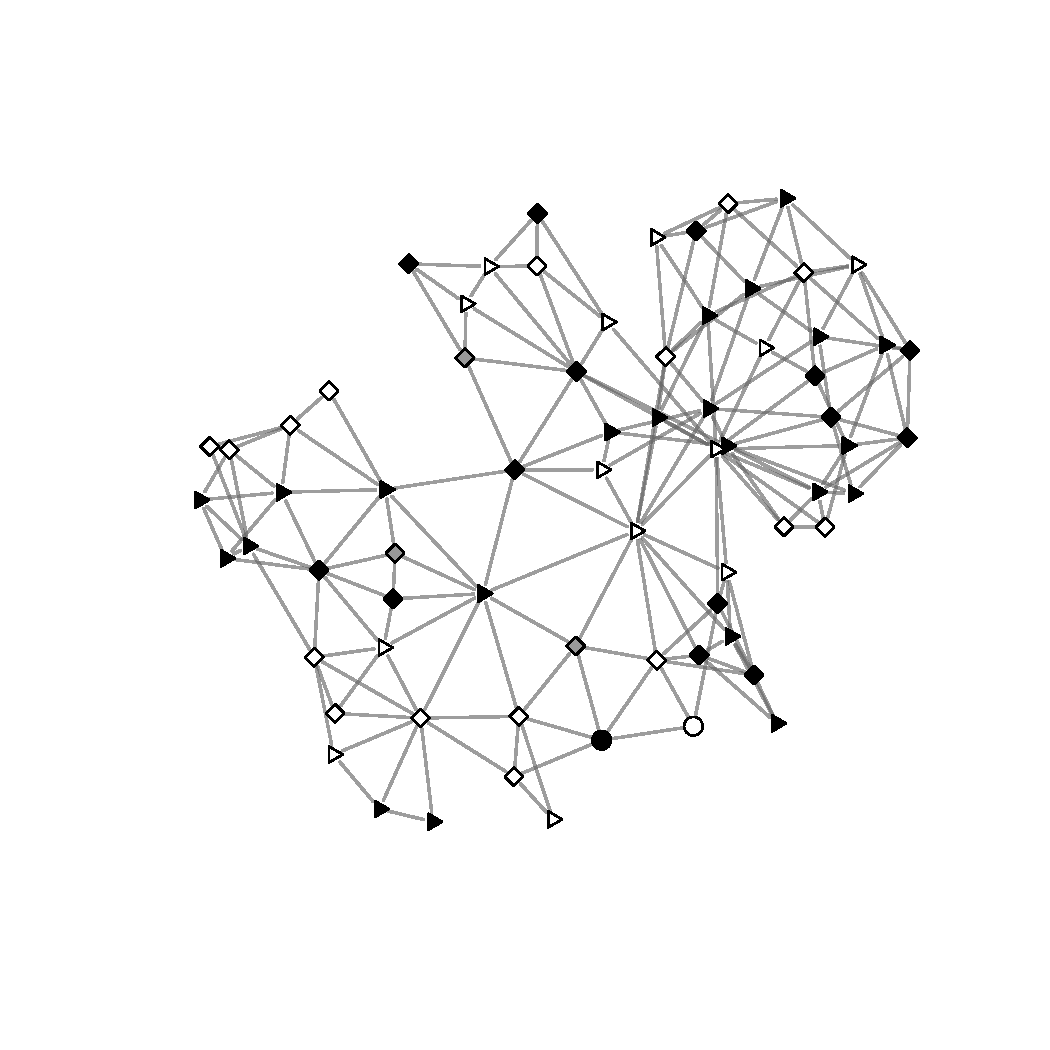
\includegraphics[scale=.55, clip=true,trim =2cm 2cm 2cm 2cm ]{./images/coppock_geographic_net.pdf} & 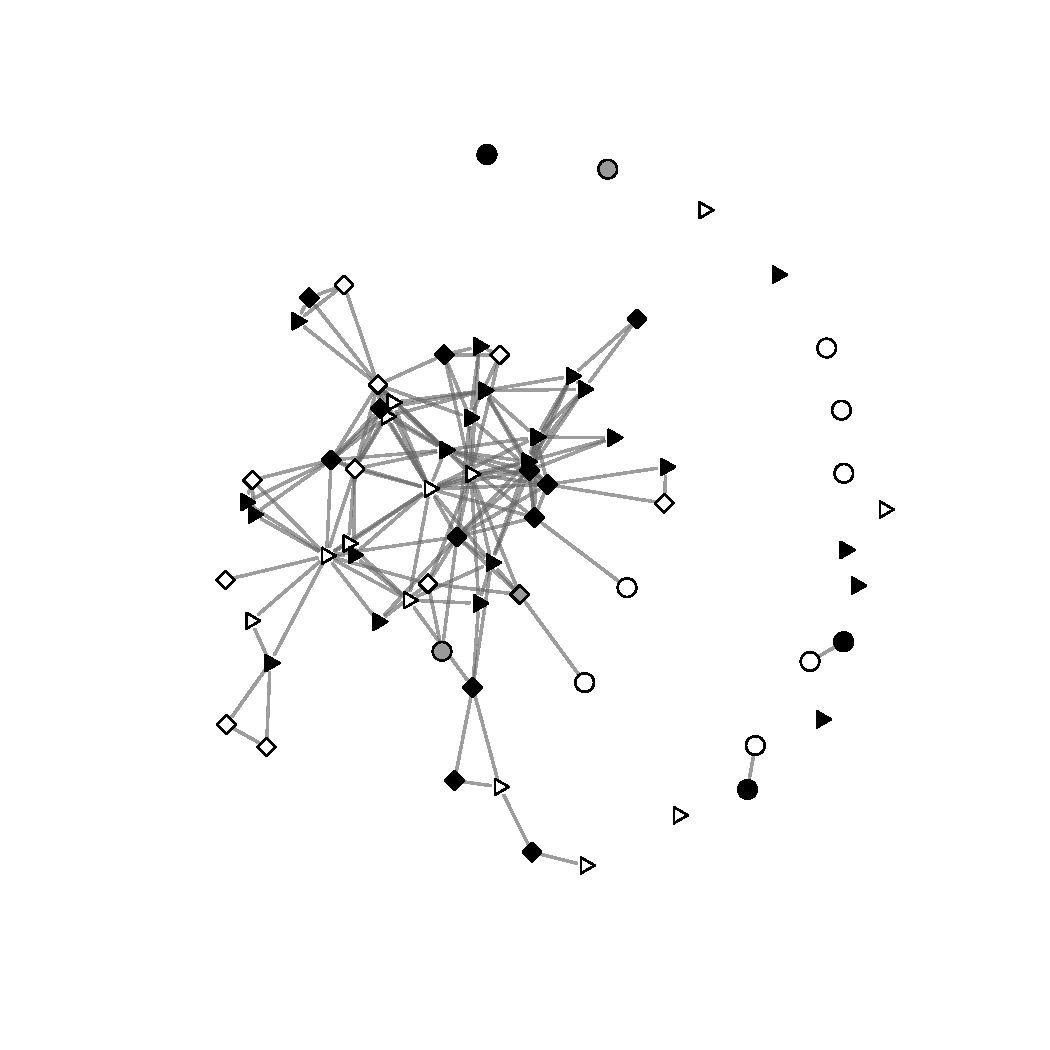
\includegraphics[scale=.55, clip=true,trim =2cm 2cm 2cm 2cm]{./images/nm_committee_net.pdf} \\ 
\end{tabular}
{\bf Ideological Network (top 5\%)} \\
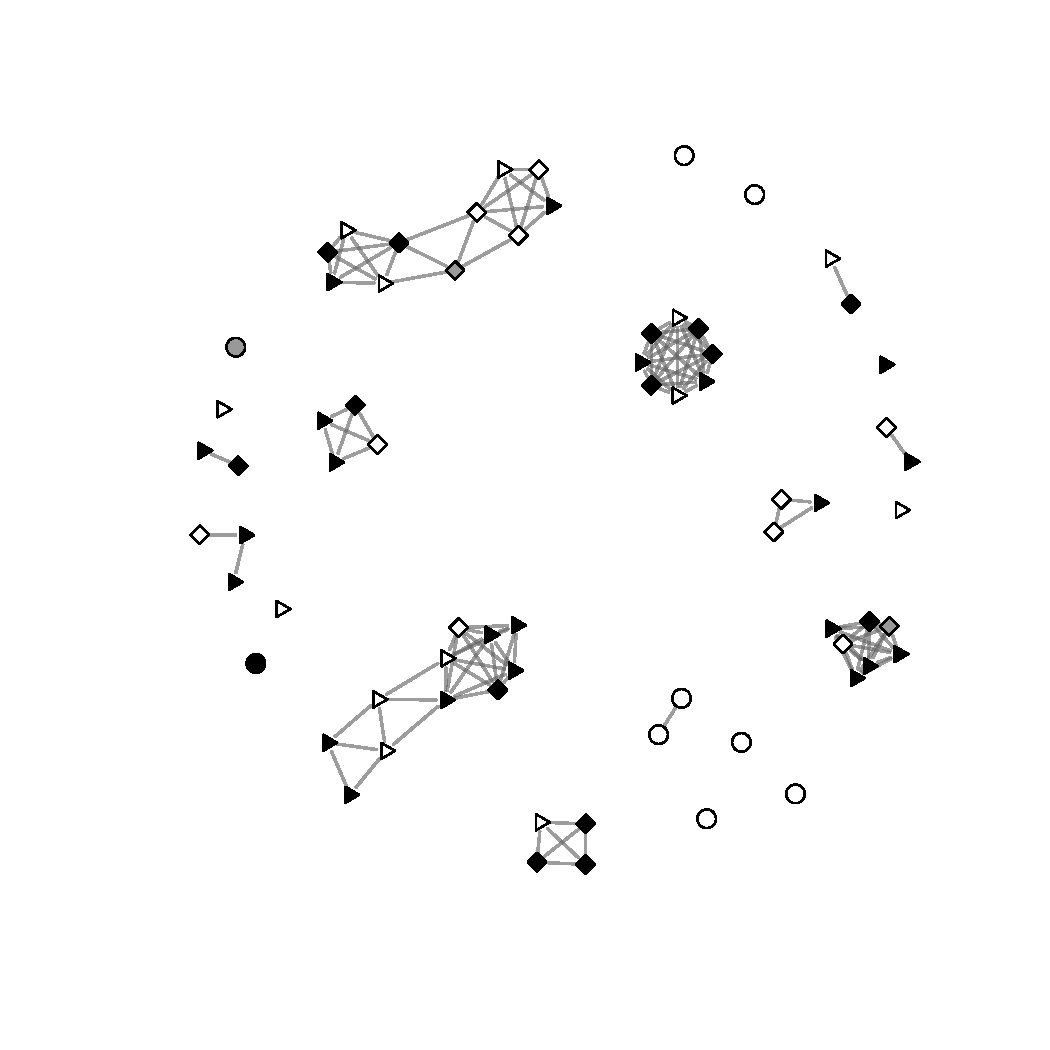
\includegraphics[scale=.55, clip=true,trim =2cm 2cm 2cm 2cm]{./images/coppock_ideological_net.pdf}
\caption{Different networks among New Mexico legislators. Colors denote outcome: black means voted with district, gray means abstained, white means voted against. Shape denotes treatment status. Triangles are treated. Squares are adjacent to treated. Circles are isolated from treatment}
\label{fig:nh-nets}
\end{figure}


\section{Appendix}
\subsection{Appendix 1A}

In this section, we will look at user-defined R-functions that replicate the Bowers et. al. methodology ( \citep{bowers2012reasoning}). There will be four steps in this:

\begin{itemize}
\item A function to transform the observed outcomes into potential outcomes for any treatment assignment w
\item A function to separate the hypothesized treatment effect
\item A function to calculate test statistic
\item A function to calculate the p-value.
\end{itemize}

The results from the ks.test function in R for calculating Kolmogorov-Smirnoff test statistic are verified with that in Footnote 12 of the paper.


\textbf{Function 1: calculating potential outcomes}

\begin{lstlisting}[language=R]
set.seed(132)
library(doParallel)
library(foreach)
library(kSamples)
library(network)
library(permute)

#### Potential outcomes ####

#### Transform uniformity trial outcome into observed outcome
unif.to.z <- function(z, S, y.0, beta, tau){
  # z: observed treatment assignment
  # S: adjacency matrix
  # y.0: outcome vector for uniformity trial
  # beta: growth curve parameter
  # tau: rate of growth parameter
  
  scalar <- as.vector(t(z)%*%S)
  spillover <- rep(NA, n)
  
  spillover <- beta + ((1-z) * (1-beta) * exp(-tau^2 * scalar))
  
  # This is equation 4
  h.y0.z <- spillover*y.0
}

#### Transform observed outcome into uniformity trial outcome
z.to.unif <- function(z, S, y.z, beta, tau){
  # z: initial treatment assignment
  # S: adjacency matrix
  # y.z: observed outcome vector
  # beta: growth curve parameter
  # tau: rate of growth parameter

  scalar <- as.vector(t(z)%*%S)
  spillover <- rep(NA, n)
  
  # Equation (3)
  spillover <- beta + ((1-z) * (1-beta) * exp(-tau^2 * scalar))
  
  # This is equation 5
  h.yz.0 <- (1/spillover)*y.z
}

#### Transform observed outcome into outcome for ANY other assignment w
z.to.w <- function(z, S, w, y.z, beta, tau){
  # z: initial treatment assignment
  # S: adjacency matrix
  # w: new treatment assignment
  # y.z: vector of outcomes for z
  # beta: growth curve parameter
  # tau: rate of growth parameter
  
  scalar.z <- as.vector(t(z)%*%S)
  scalar.w <- as.vector(t(w)%*%S)
  
  spillover.z <- rep(NA, n)
  spillover.z <- beta + ((1-z) * (1-beta) * exp(-tau^2 * scalar.z))
  
  
  spillover.w <- rep(NA, n)
  spillover.w <- beta + ((1-w) * (1-beta) * exp(-tau^2 * scalar.w))
  
  
  # Below is the actual function that transforms observed outcomes into potential outcomes
  # Equation (6)
  
  h.z.to.w <- (spillover.w / spillover.z) * y.z
}

#### Testing and p-value calculation ####

p.val <- function(z, y.z){
  
  cl <- makeCluster(4) #Setup for parallel computing
  registerDoParallel(cl)
    
  # Calculate the outcome vector after taking away the effect of treatment
  y.0 <- z.to.unif(z=z, S=S, y.z=y.z, beta=beta, tau=tau)
  
  # Calculate test statistic
  test.stat <- ks.test(y.0[z==1], y.0[z==0],
                       alternative = "g")$statistic
  sign <- noquote(strsplit(names(test.stat), NULL)[[1]])[3]
  if(sign=="+"){
    test.stat <- test.stat
  }else{
    test.stat <- test.stat*-1
  }  
  
  # Calculate a vector of test statistic using permutations
  results <- foreach (i = 1:perms) %dopar%{
    require(permute)
    perm.z <- z[sample(1:length(z),length(z),rep=F)]
    perm.test.stat <- ks.test(y.0[perm.z==1], y.0[perm.z==0],
                              alternative = "g")$statistic
    sign <- noquote(strsplit(names(perm.test.stat), NULL)[[1]])[3]
    
    if(sign=="+"){
      return(perm.test.stat)
    }else{
      return(perm.test.stat*-1)
    }
  }
  stopCluster(cl)
  
  # A vector of test statistics
  all.test.stat.vals <- unlist(results)
  
  # Calculating p-value
  pval <- sum(all.test.stat.vals > test.stat)/perms
  return(pval)
}
\end{lstlisting}


\subsection{Appendix 1B}

Below code replicates the \citep{coppock2014information} results using the framework setup in the Bowers replication code
(Version before final corrections by BD)

\begin{lstlisting}[language=R]

setwd("~/Dropbox/professional/Research/Active/causalityinnetworks-agenda/Interference_in_Field_Experiments/Analysis/coppock_replication_data/") # BD

rm(list=ls())
set.seed(312)

library(doParallel)
library(fields)
library(foreach)
library(kSamples)
library(network)
library(permute)
library(wnominate)


#### Read the original Butler and Nicketson data
#### This is the New Mexico dataset

data <- read.table("nm.replication.tab", sep="\t", header=TRUE)

z <- data$treatment #observed treatment
y.z <- data$sb24 #observed outcome
n <- length(y.z) #number of observations
t <- length(z[z==1]) #number of treated units
perms <- 10000 #number of permutations to use in generating expected exposure
perms.test <- 1000 #number of permutations used in testing


#### Generate Similarity Scores (this code taken from CoppockJEPS_datapreparation.R)

nmhouse2008 <-read.csv("CoppockJEPS_rollcalldata.csv")
bills <- data.frame(nmhouse2008[5:21])

## Nominate Scores

bills_nona <- bills
bills_nona[bills_nona==99] <- NA
rollcalls <- rollcall(bills_nona)
nominate_scores <- wnominate(rollcalls, polarity=c(1, 2), minvotes=10)
dwnom_scores <- nominate_scores$legislators$coord1D

get.similarity <- function(x, y){
  return((2-abs(x-y))/2)
}


## Create an adjacency/similarity matrix using ideology
S.ideo <- matrix(NA, ncol=70, nrow=70)
for (i in 1:70){
  for (j in 1:70){
    S.ideo[i,j] <- get.similarity(dwnom_scores[i], dwnom_scores[j])
  }
}
diag(S.ideo) <- 0
S.ideo[is.na(S.ideo)==T] <- 0


#### Generate expected exposure
perm <- replicate(perms, z[sample(1:length(z),length(z),rep=F)])

expected.exp0 <- rep(0, n)
expected.exp1 <- rep(0, n)

for(p in 1:ncol(perm)){
	zp <- perm[,p]
	for(i in 1:n){
		if (zp[i] == 1){
				expected.exp1[i] <- expected.exp1[i] + sum(S.ideo[i,-i]*zp[-i])
			}
			else{
				expected.exp0[i] <- expected.exp0[i] + sum(S.ideo[i,]*zp)
			}
	}
}
num_treat <- apply(perm,1,sum)
num_control <- apply(1-perm,1,sum)
expected.exp1 <- expected.exp1/num_treat
expected.exp0 <- expected.exp0/num_control


#### Generate expected and net exposure
#### This is the spillover effect model

indirect.treatment <- function(permutation, adj.mat){ #any treatment assignment vector and adjacency matrix can be used
  # permutation: can be the initial treatment assignment or a permutation
  raw.exp <- rep(NA, n)
  for (i in 1:n){
    raw.exp[i] <- sum(adj.mat[i,]*permutation)
    }
  
  net.exp <- raw.exp - (permutation*expected.exp1 + (1-permutation)*expected.exp0)
  standard.exp <- (net.exp - mean(net.exp))/sd(net.exp) #this is the spillover or indirect effect
  return(standard.exp)
}


#### We now model the uniformity trial transformation

z.to.unif <- function(outcome, beta1, beta2, permutation, adj.mat){
  # outcome: vector of direct treatment outcomes
  # beta1: direct treatment effect parameter
  # beta2: indirect treatment effect parameter
  # permutation: vector of a permutation of z (can be z itself)
  # adj.mat: adjacency matrix
  
  exposure <- indirect.treatment(permutation, adj.mat)
  # This is equation 5
  h.yz.0 <- outcome - (beta1*permutation) - (beta2*exposure)
  return(h.yz.0)
}


#### Testing and p-value calculation

beta1s <- seq(from=-.7, to=0.2, by=.025)
beta2s <- seq(from=-.7, to=0.2, by=.025)

pvals <- matrix(NA, length(beta1s), length(beta2s))

cl <- makeCluster(4) #Setup for parallel computing
registerDoParallel(cl)

pvalues.ideology <- foreach (i = 1:length(beta1s)) %do% {
  abc <- foreach (j = 1:length(beta2s)) %do% {
    
    # Calculate the outcome vector after taking away the effect of treatment
    y.0 <- z.to.unif(outcome = y.z, beta1 = beta1s[i], beta2 = beta2s[j], permutation = z, adj.mat = S.ideo)
    
    # Calculate observed test statistic
    exposure <- indirect.treatment(permutation = z, adj.mat = S.ideo)
    test.stat <- sum((lm(y.0 ~ z + exposure, na.action = na.omit)$resid)^2)
    
    # Calculate a vector of test statistic using permutations
    
    results <- foreach (k = 1:perms.test) %dopar% {
      require(permute)
      perm.z <- z[sample(1:length(z),length(z),rep=F)] #Each time we sample a permutation of z
      perm.y.0 <- z.to.unif(outcome = y.z, beta1 = beta1s[i], beta2 = beta2s[j], permutation = perm.z, adj.mat = S.ideo)
      perm.exposure <- indirect.treatment(permutation = perm.z, adj.mat = S.ideo)
      
      perm.test.stat <- sum((lm(perm.y.0 ~ perm.z + perm.exposure, na.action = na.omit)$resid)^2)
      }
    
    
    # A vector of test statistics
    all.test.stat.vals <- as.numeric(unlist(results))
    
    # Calculating p-value
    pval <- sum(all.test.stat.vals < test.stat)/perms.test
  }
  as.numeric(unlist(abc))
}

stopCluster(cl)

for (i in 1:length(beta1s)){
  pvals[i,] <- unlist(pvalues.ideology[i])
}

pvals


## Creating a plot
image.plot(beta1s, beta2s, pvals,
           main = "Plot of p-values", xlab = "Direct effects", ylab = "Indirect effects")

pdf("pvalues_figure.pdf")
image.plot(beta1s, beta2s, pvals,
           main = "Plot of p-values",
           xlab = "Direct effects", ylab = "Indirect effects")
dev.off()


\end{lstlisting}


%===================References======================
\clearpage
\bibliographystyle{apsr}
\bibliography{cause_and_networks}




\end{document}
